\textit{Definition:} DO type identification statistics is a random variable of the type of the left part of the rule (2).

To evaluate the efficiency of the algorithm, it is naturally necessary to know the law of probability distribution of the recognition statistics, the threshold level for deciding on the type of the detected DO and the stability properties of the law.

Obviously, from the structure of the left-hand side of (2), the law can be established subject to the known laws of the distribution of the probabilities of each of its terms as sufficient statistics. The laws of the terms are conditional: they are established provided that DO are located in the OED control zone for each alternative type.

The terms are the functions of samples of independent measurements of the coordinates of the elevation angle of either the azimuth or the distance in the time interval for detecting the DO by OED.

Under such circumstances, a formal solution to the problem of restoring the desired law of statistics of the form of the left part (2) as a linear combination is reduced to performing the sequence of the following operations for the measurement samples and the functions of them:

Under such circumstances, a formal solution to the problem of restoring the desired law of statistics of the form of the left part (2) as a linear combination is reduced to performing the sequence of the following operations for the measurement samples and the functions of them:

1. Conversion of samples to the form of primary sufficient statistics: fractal dimensions $d(\theta)$, $d(\varphi)$, $d(D)$, wavelet spectral energy  $ u(w(\theta)) $, $ u(w(\varphi)) $, $ u(w(D)) $ and maximum eigenvalues $ \lambda(\theta) $, $ \lambda(\varphi) $, $ \lambda(D) $  . The transformation is carried out by algorithmically realized linear functionals and operators, their substantive essence is disclosed in the previous subsection.

2. Calculation of the laws of probability distribution of sufficient statistics $d(\theta)$, $d(\varphi)$, $d(D)$, $ u(w(\theta)) $, $ u(w(\varphi)) $,  $ \lambda(\theta) $, $ \lambda(\varphi) $, $ \lambda(D) $.

The type of laws for various conditions - the types of DO, observed by the ODE, is set by modeling, their mathematical description is presented in [1]. These are beta distributions with appropriate parameters for alternative DO types.

3. Calculation of probability distribution laws for function statistics

\begin{equation*}
({{p}_{j}}-1)\ln (d(\theta )-{{\mu }_{j0}}),\ ...\ ({{q}_{j}}-1)\ln ({{\mu }_{j1}}-d(\theta )),
\end{equation*}

\begin{equation*}
({{p}_{j}}-1)\ln (d(\varphi )-{{\mu }_{j0}}),\ ...\ ({{q}_{j}}-1)\ln ({{\mu }_{j1}}-d(\varphi )),
\end{equation*}

\begin{equation*}
({{p}_{j}}-1)\ln (d(D)-{{\mu }_{j0}}),\ ...\ ({{q}_{j}}-1)\ln ({{\mu }_{j1}}-d(D)),
\end{equation*}

\begin{equation*}
({{p}_{j}}-1)\ln (u(w(\theta ))-{{\mu }_{j0}}),\ ...\ ({{q}_{j}}-1)\ln ({{\mu }_{j1}}-u(w(\theta ))),
\end{equation*}

\begin{equation*}
({{p}_{j}}-1)\ln (u(w(\varphi ))-{{\mu }_{j0}}),\ ...\ ({{q}_{j}}-1)\ln ({{\mu }_{j1}}-u(w(\varphi ))),
\end{equation*}

\begin{equation*}
({{p}_{j}}-1)\ln (u(w(D))-{{\mu }_{j0}}),\ ...\ ({{q}_{j}}-1)\ln ({{\mu }_{j1}}-u(w(D))),
\end{equation*}

\begin{equation*}
({{p}_{j}}-1)\ln (\lambda (\theta ))-{{\mu }_{j0}}),\ ...\ ({{q}_{j}}-1)\ln ({{\mu }_{j1}}-\lambda (\theta )),
\end{equation*}

\begin{equation*}
({{p}_{j}}-1)\ln (\lambda (\varphi ))-{{\mu }_{j0}}),\ ...\ ({{q}_{j}}-1)\ln ({{\mu }_{j1}}-\lambda (\varphi )),
\end{equation*}

\begin{equation*}
({{p}_{j}}-1)\ln (\lambda (D))-{{\mu }_{j0}}),\ ...\ ({{q}_{j}}-1)\ln ({{\mu }_{j1}}-\lambda (D)).
\end{equation*}

The laws are calculated using the well-known formula $ \psi (y)=f(\phi (y))\left| {\phi }'(y) \right| $, where $ y=\xi (x) $, $ \xi $ is a differentiable monotonic function, $ \varphi $ is an inverse function with respect to a function  $ \xi $, is a density of a random variable $ y $, $f(x|{{s}_{j}})$ a density of a random variable  subject to the condition $ {{s}_{j}} $ of the DO type.

In the case, for the component, $({{p}_{j}}-1)\ln [u(w(\theta ))-{{\mu }_{j0}}]$ taking into account the notation in the formula for $\psi (y)$ have $y=({{p}_{j}}-1)\ln (u(w(\theta ))-{{\mu }_{j0}})$ or this $x=u(w(\theta ))=\exp \{y/({{p}_{j}}-1)\}+{{\mu }_{j0}}=\phi (y)$ is  a random variable with a beta-distribution density ($\theta $ - designation of the non-random elevation position) and the probability distribution density of a random variable has the form.


\begin{equation*}
\begin{gathered}
\psi (y|{{s}_{j}})=f(\phi (y|{{s}_{j}})\left| {\phi }'(y) \right|=f(\exp \{y/({{p}_{j}}-1)\}+{{\mu }_{i0}})\left| (1/({{p}_{j}}-1))\exp \{y/({{p}_{j}}-1)\} \right|= \\ 
  =\frac{\left| (1/({{p}_{j}}-1)) \right|\exp \{y/({{p}_{j}}-1)\}}{({{\mu }_{j1}}-{{\mu }_{j0}})}\frac{\Gamma ({{p}_{j}}+{{q}_{j}})}{\Gamma ({{p}_{j}})\Gamma ({{q}_{j}})} \times \\
\times {{\left( \frac{\exp \{y/({{p}_{j}}-1)\}+{{\mu }_{i0}}}{{{\mu }_{j1}}-{{\mu }_{j0}}} \right)}^{{{p}_{j}}-1}}{{\left( 1-\frac{\exp \{y/({{p}_{j}}-1)\}+{{\mu }_{j0}}}{{{\mu }_{j1}}-{{\mu }_{j0}}} \right)}^{{{q}_{j}}-1}} \\ 
\end{gathered}
\end{equation*}


Below we will consider the option $u(w(\theta ))\in [{{\mu }_{j0}}=0,{{\mu }_{j1}}=1]$. The density $\psi (y|{{s}_{j}})$ will be determined only on the negative semi-axis of the values, that is, on the interval - $\infty \le \ y=\left| {{p}_{j}}-1 \right|\ln (u(w(\theta )))\le \ 0$,

\begin{equation*}
\begin{gathered}
\psi (\left. y \right|{{s}_{j}})=(1/\left| {{p}_{j}}-1 \right|)\exp \{y/\left| {{p}_{j}}-1 \right|\}\frac{\Gamma ({{p}_{j}}+{{q}_{j}})}{\Gamma ({{p}_{j}})\Gamma ({{q}_{j}})}{{\left( \exp \{y/\left| {{p}_{j}}-1 \right|\} \right)}^{{{p}_{j}}-1}}{{\left( 1-\exp \{y/\left| {{p}_{j}}-1 \right|\} \right)}^{{{q}_{j}}-1}}
\end{gathered}
\end{equation*}

and we can see all other random variables type $\left| {{p}_{i}}-1 \right|\ln u(w(\theta ))$ will have the same type of density, derived from (1).

Acting in a similar way, we obtain the conditional probability density distribution of random variables of the type $\nu =\left| {{q}_{j}}-1 \right|\ln [1-u(w(\theta ))]$; density is written as

\begin{equation*}
\begin{gathered}
\psi (\left. \nu  \right|{{s}_{j}})=f(\phi (\left. \nu  \right|{{s}_{j}})\left| \phi '(\nu ) \right|=f(1-\exp \left\{ {\nu }/{\left| {{q}_{j}}-1 \right|}\; \right\})\left| ({1}/{\left| {{q}_{j}}-1 \right|)\exp \left\{ {\nu }/{\left| {{q}_{j}}-1 \right|}\; \right\}}\; \right|
\end{gathered}
\end{equation*}

and given that $f({{\mu }_{j1}}-\exp \{\nu /({{q}_{j}}-1)\}$ is a beta distribution, in the form

\begin{equation*}
\begin{gathered}
\psi (\left. \nu  \right|{{s}_{j}})=(1/\left| {{q}_{j}}-1 \right|)\exp \{\nu /\left| {{q}_{j}}-1 \right|\}\frac{\Gamma ({{p}_{j}}+{{q}_{j}})}{\Gamma ({{p}_{j}})\Gamma ({{q}_{j}})} \times \\
\times {{\left( 1-\exp \{\nu /\left| {{q}_{j}}-1 \right|\} \right)}^{{{p}_{j}}-1}}{{\left( \exp \{\nu /\left| {{q}_{j}}-1 \right|\} \right)}^{{{q}_{j}}-1}}.
\end{gathered}
\end{equation*}

and note that the laws obtained $\psi (y|{{s}_{j}})$ and $\psi (\nu |{{s}_{j}})$ do not preserve the form of the beta law: they describe random variables $y$ and$\nu $, taking values from an interval $(-\infty ,0)$.

4. Calculation of probability distribution laws for statistics of functions of the form

\begin{equation*}
({{p}_{j}}-1)\ln (d(\theta )-{{\mu }_{j0}})-({{p}_{i}}-1)\ln (d(\theta )-{{\mu }_{i0}}),\ ...\ ({{q}_{j}}-1)\ln ({{\mu }_{j1}}-d(\theta ))-({{q}_{i}}-1)\ln ({{\mu }_{i1}}-d(\theta ))
\end{equation*}

\begin{equation*}
({{p}_{j}}-1)\ln (d(\varphi )-{{\mu }_{j0}})-({{p}_{i}}-1)\ln (d(\varphi )-{{\mu }_{i0}}),\ ...\ ({{q}_{j}}-1)\ln ({{\mu }_{j1}}-d(\varphi ))-({{q}_{i}}-1)\ln ({{\mu }_{i1}}-d(\varphi ))
\end{equation*}

\begin{equation*}
({{p}_{j}}-1)\ln (d(D)-{{\mu }_{j0}})-({{p}_{i}}-1)\ln (d(D)-{{\mu }_{i0}}),\ ...\ ({{q}_{j}}-1)\ln ({{\mu }_{j1}}-d(D))-({{q}_{i}}-1)\ln ({{\mu }_{i1}}-d(D))
\end{equation*}

\begin{equation*}
\begin{gathered}
({{p}_{j}}-1)\ln (u(w(\theta ))-{{\mu }_{j0}})-({{p}_{i}}-1)\ln (u(w(\theta ))-{{\mu }_{i0}}),\ ...\ ({{q}_{j}}-1)\ln ({{\mu }_{j1}}-u(w(\theta )))- \\
- ({{q}_{i}}-1)\ln ({{\mu }_{i1}}-u(w(\theta )))
\end{gathered}
\end{equation*}

\begin{equation*}
\begin{gathered}
({{p}_{j}}-1)\ln (u(w(\varphi ))-{{\mu }_{j0}})-({{p}_{i}}-1)\ln (u(w(\varphi ))-{{\mu }_{i0}}),\ ...\ ({{q}_{j}}-1)\ln ({{\mu }_{j1}}-u(w(\varphi )))- \\
- ({{q}_{i}}-1)\ln ({{\mu }_{i1}}-u(w(\varphi )))
\end{gathered}
\end{equation*}

\begin{equation*}
\begin{gathered}
({{p}_{j}}-1)\ln (u(w(D))-{{\mu }_{j0}})-({{p}_{i}}-1)\ln (u(w(D))-{{\mu }_{i0}}),\ ...\ ({{q}_{j}}-1)\ln ({{\mu }_{j1}}-u(w(D)))- \\
- ({{q}_{i}}-1)\ln ({{\mu }_{i1}}-u(w(D)))
\end{gathered}
\end{equation*}

\begin{equation*}
({{p}_{j}}-1)\ln (\lambda (\theta )-{{\mu }_{j0}})-({{p}_{i}}-1)\ln (\lambda (\theta )-{{\mu }_{i0}}),\ ...\ ({{q}_{j}}-1)\ln ({{\mu }_{j1}}-\lambda (\theta ))-({{q}_{i}}-1)\ln ({{\mu }_{i1}}-\lambda (\theta ))
\end{equation*}

\begin{equation*}
({{p}_{j}}-1)\ln (\lambda (\varphi )-{{\mu }_{j0}})-({{p}_{i}}-1)\ln (\lambda (\varphi )-{{\mu }_{i0}}),\ ...\ ({{q}_{j}}-1)\ln ({{\mu }_{j1}}-\lambda (\varphi ))-({{q}_{i}}-1)\ln ({{\mu }_{i1}}-\lambda (\varphi ))
\end{equation*}

\begin{equation*}
({{p}_{j}}-1)\ln (\lambda (D)-{{\mu }_{j0}})-({{p}_{i}}-1)\ln (\lambda (D)-{{\mu }_{i0}}),\ ...\ ({{q}_{j}}-1)\ln ({{\mu }_{j1}}-\lambda (D))-({{q}_{i}}-1)\ln ({{\mu }_{i1}}-\lambda (D))
\end{equation*}

and establishing the properties of the distribution laws of these statistics for ${{\mu }_{j0}}=0,\text{ }{{\mu }_{j1}}=1$.

It can be seen that the probability densities of differences of equally distributed random variables should be calculated, compared with (1) for the alternative DO types of  ${{s}_{j}}$ and ${{s}_{i}}$. To do this, we use the formula of the composition of the laws of the distribution of independent random variables. $\left| {{p}_{j}}-1 \right|\ln u(w(\theta ))$ and $\left| {{p}_{i}}-1 \right|\ln u(w(\theta ))$.

The desired density is

\begin{equation*}
{{g}_{y-\nu }}({{z}_{1}}|{{s}_{j}},{{s}_{i}})=\int\limits_{\min \{y\}}^{\max \{y\}}{{{\psi }_{Y}}(y|{{s}_{j}}){{\psi }_{\nu }}((y-{{z}_{1}})|{{s}_{i}})dy}
\end{equation*}

where ${{z}_{1}}=y-\nu =\left| {{p}_{j}}-1 \right|\ln u(w(\theta ))-\left| {{p}_{i}}-1 \right|\ln u(w(\theta ))$ and for ${{\mu }_{j0}}=0,\ {{\mu }_{j1}}=1$ and ${{\mu }_{i0}}=0,\ {{\mu }_{i1}}=1\quad u(w(\theta )\in \left[ 0,1 \right]$, density of sufficient statistics $y$ and $\nu $ for DO types $j,i=1,2,\ ...\ ,M,\ j\ne i$, are not equal to zero in the intervals $-\infty \le \left| {{p}_{j}}-1 \right|\ln u(w(\theta ))\le 0$, $-\infty \le \left| {{p}_{i}}-1 \right|\ln u(w(\theta ))\le 0$ for each $j$, $i$. In this case, the density ${{\psi }_{y}}(y|{{s}_{j}})$ is nonzero at $-\infty \le y\le 0$, and the density ${{\psi }_{\nu }}((y-{{z}_{1}})|{{s}_{i}})$ is nonzero at $y-{{z}_{1}}\le 0$ or $y\le {{z}_{1}}$, $-\infty \le {{z}_{1}}\le \infty $, the statistics is unlimited and the required density is written in such convolutions:

as ${{z}_{1}}\le 0$ ${{g}_{y-\nu }}({{z}_{1}}|{{s}_{j}},{{s}_{i}})=\int\limits_{-{{\infty }_{1}}}^{-{{z}_{1}}}{{{\psi }_{Y}}(y|{{s}_{j}}){{\psi }_{\nu }}((y-{{z}_{1}})|{{s}_{i}})dy},$

and as ${{z}_{1}}>0$ ${{g}_{y-\nu }}({{z}_{1}}|{{s}_{j}},{{s}_{i}})=\int\limits_{-\infty }^{0}{{{\psi }_{Y}}(y|{{s}_{j}}){{\psi }_{\nu }}((y-{{z}_{1}})|{{s}_{i}})dy},$

where 

\begin{equation*}
\begin{gathered}
 {{\psi }_{Y}}(y|{{s}_{j}}){{\psi }_{\nu }}((y-{{z}_{1}})|{{s}_{i}})= \\ 
  =\left| \frac{1}{{{p}_{j}}-1} \right|\exp \{y/\left| {{p}_{j}}-1 \right|\}\frac{\Gamma ({{p}_{j}}+{{q}_{j}})}{\Gamma ({{p}_{j}})\Gamma ({{q}_{j}})}{{\left( \exp \{y/\left| {{p}_{j}}-1 \right|\} \right)}^{{{p}_{j}}-1}}{{\left( 1-\exp \{y/\left| {{p}_{j}}-1 \right|\} \right)}^{{{q}_{j}}-1}}\times  \\ 
  \times \left| \frac{1}{{{p}_{i}}-1} \right|\exp \{(y-{{z}_{1}})/\left| {{p}_{i}}-1 \right|\}\frac{\Gamma ({{p}_{i}}+{{q}_{i}})}{\Gamma ({{p}_{i}})\Gamma ({{q}_{i}})}{{\left( 1-\exp \{(y-{{z}_{1}})/\left| {{p}_{i}}-1 \right|\} \right)}^{{{p}_{i}}-1}}{{\left( \exp \{(y-{{z}_{1}})/\left| {{p}_{i}}-1 \right|\} \right)}^{{{q}_{i}}-1}}
\end{gathered}
\end{equation*}

Convolutions of the same type of distribution. It is known (for example, \cite{bib_18}) that such convolutions lead to the same type of distribution. 

Due to the complexity of the expression for ${{\psi }_{Y}}(y|{{s}_{j}}){{\psi }_{\nu }}((y-{{z}_{1}})|{{s}_{i}})$ obtaining an analytical solution, convolutions are practically difficult. The Laplace transform is also difficult to compute for the analytical expression of the desired law. Therefore, we use numerical integration using the MatLab trapz function.
In Fig.~\ref{fig:fig_2}, Fig.~\ref{fig:fig_3}, Fig.~\ref{fig:fig_4}, a graphic representation of the laws numerically obtained for different pairs of parameters are given $\left\{ {{p}_{j}},{{q}_{j}} \right\}$; the latter are given in table \ref{tab:table_1} [1]. 

\begin{table}[]
\centering
\caption{Parameter values $\left\{ {{p}_{j}},{{q}_{j}} \right\}$}
\label{tab:table_1}
\begin{tabular}{|c|c|C{0.1\textwidth}|C{0.1\textwidth}|C{0.1\textwidth}|C{0.1\textwidth}|C{0.12\textwidth}|C{0.1\textwidth}|}
\hline
\multirow{2}{*}{\begin{tabular}[c]{@{}c@{}}Measured\\ coordinates\end{tabular}} & \multirow{2}{*}{\begin{tabular}[c]{@{}c@{}}DO\\ type\end{tabular}} & \multicolumn{2}{c|}{\begin{tabular}[c]{@{}c@{}}Parameters for the $ \beta $\\ - distribution\\ of fractal dimension\end{tabular}} & \multicolumn{2}{c|}{\begin{tabular}[c]{@{}c@{}}Parameters for the $ \beta $\\  - distribution of\\ maximum eigenvalue\end{tabular}} & \multicolumn{2}{c|}{\begin{tabular}[c]{@{}c@{}}Parameters for the $ \beta $\\  - distribution of\\ energy of wavelet spectrum\end{tabular}} \\ \cline{3-8} 
 &  & p & q & p & q & p & q \\ \hline
\multirow{3}{*}{Range} & 1 & 0.64 & 0.88 & 0.64 & 0.64 & 0.73 & 1.47 \\ \cline{2-8} 
 & 2 & 0.73 & 1.47 & 1.08 & 4.32 & 0.46 & 0.46 \\ \cline{2-8} 
 & 3 & 0.46 & 0.46 & 1.00 & 5.65 & 0.76 & 2.29 \\ \hline
\multirow{3}{*}{Azimuth} & 1 & 1.02 & 3.58 & 0.64 & 0.64 & 0.92 & 2.01 \\ \cline{2-8} 
 & 2 & 1.01 & 2.63 & 1.09 & 3.27 & 0.83 & 1.38 \\ \cline{2-8} 
 & 3 & 0.60 & 0.60 & 1.05 & 2.45 & 0.57 & 0.57 \\ \hline
\multirow{3}{*}{\begin{tabular}[c]{@{}c@{}}Elevation\\ angle\end{tabular}} & 1 & 1.13 & 5.07 & 1.08 & 4.32 & 1.13 & 5.07 \\ \cline{2-8} 
 & 2 & 1.07 & 2.30 & 1.00 & 5.65 & 0.90 & 1.29 \\ \cline{2-8} 
 & 3 & 0.66 & 0.66 & 0.64 & 0.64 & 0.66 & 0.66 \\ \hline
\end{tabular}
\end{table}

From the representations of the laws in Fig.~\ref{fig:fig_2}, Fig.~\ref{fig:fig_3}, Fig.~\ref{fig:fig_4} that they are characterized by the following properties: they are continuous, single-vertex, have a single (each its own) mode, are differentiable everywhere except for (for some densities) a single point - the argument corresponding to the top of the law that the derivatives of the laws do not decrease to the left of the arguments vertices and do not increase to the right. The laws are defined on areas as areas of attraction, they are symmetric (the asymmetry of some graphs is due to the nonoptimality of the choice of the integration step in the Matlab system), they have finite dispersions and can be approximated only by the density of the Laplace law. The latter are infinitely divisible and limit for the sum of independent identically distributed random variables \cite{bib_12, bib_17}.

In this case, such a sum is the left side of expression (2). According to these features, the properties of the density of the laws of probability distribution of recognition statistics, are stable \cite{bib_18}.

Similar graphical representations and properties determine the laws of the statistics of the form $({{q}_{j}}-1)\ln ({{\mu }_{j1}}-d(\theta ))-({{q}_{i}}-1)\ln ({{\mu }_{i1}}-d(\theta ))$, that is, the statistics functions of the fractal dimension, the maximum eigenvalue and the wavelet spectrum of measurements of the coordinates of the elevation angle, azimuth and distance of the detected DO by OED.

Such statistics are taken into account in the next subparagraph.

5. Calculation of probability distribution laws for statistics sums
\begin{equation*}
({{p}_{j}}-1)\ln (d(\theta )-{{\mu }_{j0}})-({{p}_{i}}-1)\ln (d(\theta )-{{\mu }_{i0}})+({{q}_{j}}-1)\ln ({{\mu }_{j1}}-d(\theta ))-({{q}_{i}}-1)\ln ({{\mu }_{i1}}-d(\theta ))
\end{equation*}

\begin{equation*}
({{p}_{j}}-1)\ln (d(\varphi )-{{\mu }_{j0}})-({{p}_{i}}-1)\ln (d(\varphi )-{{\mu }_{i0}})+({{q}_{j}}-1)\ln ({{\mu }_{j1}}-d(\varphi ))-({{q}_{i}}-1)\ln ({{\mu }_{i1}}-d(\varphi ))
\end{equation*}

\begin{equation*}
({{p}_{j}}-1)\ln (d(D)-{{\mu }_{j0}})-({{p}_{i}}-1)\ln (d(D)-{{\mu }_{i0}})+({{q}_{j}}-1)\ln ({{\mu }_{j1}}-d(D))-({{q}_{i}}-1)\ln ({{\mu }_{i1}}-d(D))
\end{equation*}

\begin{equation*}
\begin{gathered}
({{p}_{j}}-1)\ln (u(w(\theta ))-{{\mu }_{j0}})-({{p}_{i}}-1)\ln (u(w(\theta ))-{{\mu }_{i0}})+({{q}_{j}}-1)\ln ({{\mu }_{j1}}-u(w(\theta )))- \\
- ({{q}_{i}}-1)\ln ({{\mu }_{i1}}-u(w(\theta )))
\end{gathered}
\end{equation*}

\begin{equation*}
\begin{gathered}
({{p}_{j}}-1)\ln (u(w(\varphi ))-{{\mu }_{j0}})-({{p}_{i}}-1)\ln (u(w(\varphi ))-{{\mu }_{i0}})+({{q}_{j}}-1)\ln ({{\mu }_{j1}}-u(w(\varphi )))- \\
- ({{q}_{i}}-1)\ln ({{\mu }_{i1}}-u(w(\varphi )))
\end{gathered}
\end{equation*}

\begin{equation*}
\begin{gathered}
({{p}_{j}}-1)\ln (u(w(D))-{{\mu }_{j0}})-({{p}_{i}}-1)\ln (u(w(D))-{{\mu }_{i0}})+({{q}_{j}}-1)\ln ({{\mu }_{j1}}-u(w(D)))- \\
- ({{q}_{i}}-1)\ln ({{\mu }_{i1}}-u(w(D)))
\end{gathered}
\end{equation*}

\begin{equation*}
({{p}_{j}}-1)\ln (\lambda (\theta )-{{\mu }_{j0}})-({{p}_{i}}-1)\ln (\lambda (\theta )-{{\mu }_{i0}})+({{q}_{j}}-1)\ln ({{\mu }_{j1}}-\lambda (\theta ))-({{q}_{i}}-1)\ln ({{\mu }_{i1}}-\lambda (\theta ))
\end{equation*}

\begin{equation*}
({{p}_{j}}-1)\ln (\lambda (\varphi )-{{\mu }_{j0}})-({{p}_{i}}-1)\ln (\lambda (\varphi )-{{\mu }_{i0}})+({{q}_{j}}-1)\ln ({{\mu }_{j1}}-\lambda (\varphi ))-({{q}_{i}}-1)\ln ({{\mu }_{i1}}-\lambda (\varphi ))
\end{equation*}

\begin{equation*}
({{p}_{j}}-1)\ln (\lambda (D)-{{\mu }_{j0}})-({{p}_{i}}-1)\ln (\lambda (D)-{{\mu }_{i0}})+({{q}_{j}}-1)\ln ({{\mu }_{j1}}-\lambda (D))-({{q}_{i}}-1)\ln ({{\mu }_{i1}}-\lambda (D))
\end{equation*}

The calculation of the laws for the written amounts of random variables is also established using the composition theorem \cite{bib_14} of the laws of distribution of the differences of random variables, compiled in the previous subparagraph 4.

So, for the sum $z={{z}_{1}}+{{z}_{2}}$, in which with ${{\mu }_{j0}}=0,\ {{\mu }_{j1}}=1$ and ${{\mu }_{i0}}=0,\ {{\mu }_{i1}}=1$ with the terms ${{z}_{1}}=\left| {{p}_{j}}-1 \right|\ln u(w(\theta ))-\left| {{p}_{i}}-1 \right|\ln u(w(\theta ))$ and ${{z}_{2}}=\left| {{q}_{j}}-1 \right|\ln u(w(\theta ))-\left| {{q}_{i}}-1 \right|\ln u(w(\theta ))$, and for similar other sums of random variables, as can be seen directly from the above expressions, the distribution law is established by the formula.

\begin{equation*}
{{g}_{{{z}_{1}}+{{z}_{2}}}}(z|{{s}_{j}},{{s}_{i}})=\int\limits_{\min \{{{z}_{1}}\}}^{\max \{{{z}_{1}}\}}{{{\psi }_{{{z}_{1}}}}({{z}_{1}}|{{s}_{j}},{{s}_{i}}){{\psi }_{{{z}_{2}}}}(z-{{z}_{1}}|{{s}_{j}},{{s}_{i}})d{{z}_{1}}}
\end{equation*}

where the type of laws ${{\psi }_{{{z}_{1}}}}({{z}_{1}}|{{s}_{j}},{{s}_{i}})$ and ${{\psi }_{{{z}_{2}}}}(z-{{z}_{1}}|{{s}_{j}},{{s}_{i}})$ is defined in subparagraph 4 and presented in Fig.~\ref{fig:fig_2}, and the limits of integration can be calculated by the intervals of values  ,   of random variables, as indicated in the figures.

The laws of the form ${{g}_{{{z}_{1}}+{{z}_{2}}}}(z|{{s}_{j}},{{s}_{i}})$ are convolutions of stable single-type distributions (Fig.~\ref{fig:fig_2}), they are reduced to the same form and have the same properties as the laws of random variables ${{z}_{1}}$ and ${{z}_{2}}$. 

Hence the conclusion: the law of probability distribution of recognition statistics of DO type according to the rule of the form (2), which implements the corresponding particular algorithm (1), has the properties of stable distributions. 


\begin{figure}[h]
\setcaptionmargin{5mm}
\onelinecaptionstrue
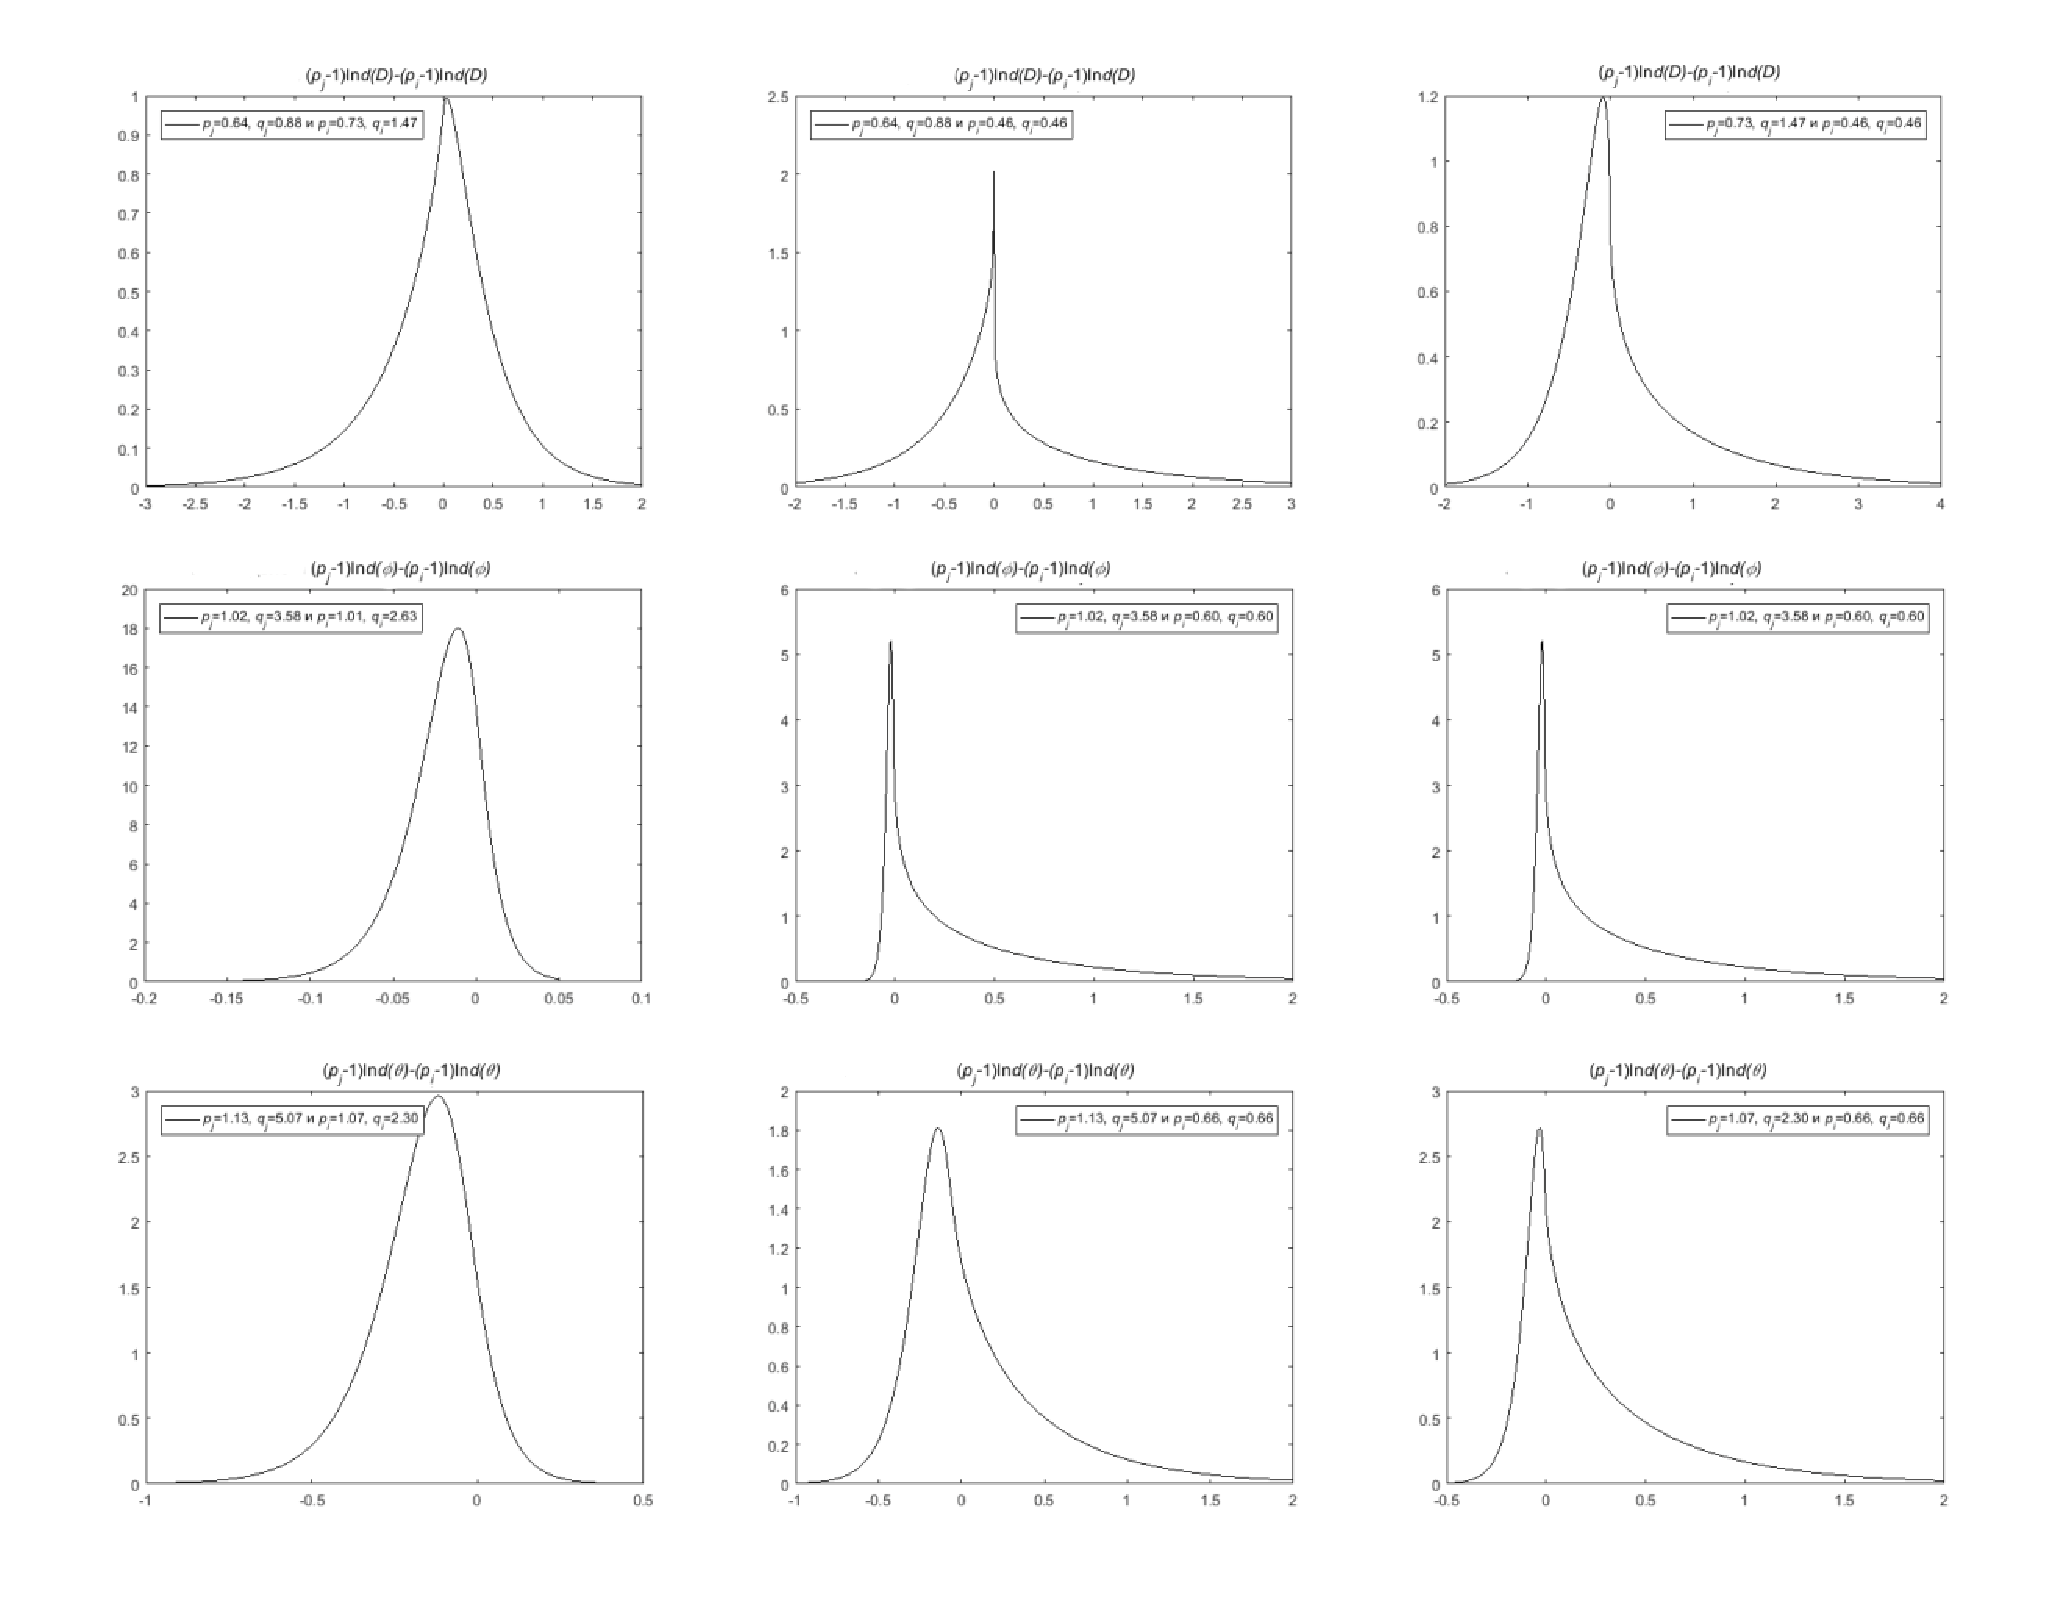
\includegraphics[width=1.0\textwidth]{pics/fig_2.pdf}
\captionstyle{normal}\caption{The laws of the distribution of statistics functions of fractal dimension.}\label{fig:fig_2}
\end{figure}

\begin{figure}[h]
\setcaptionmargin{5mm}
\onelinecaptionstrue
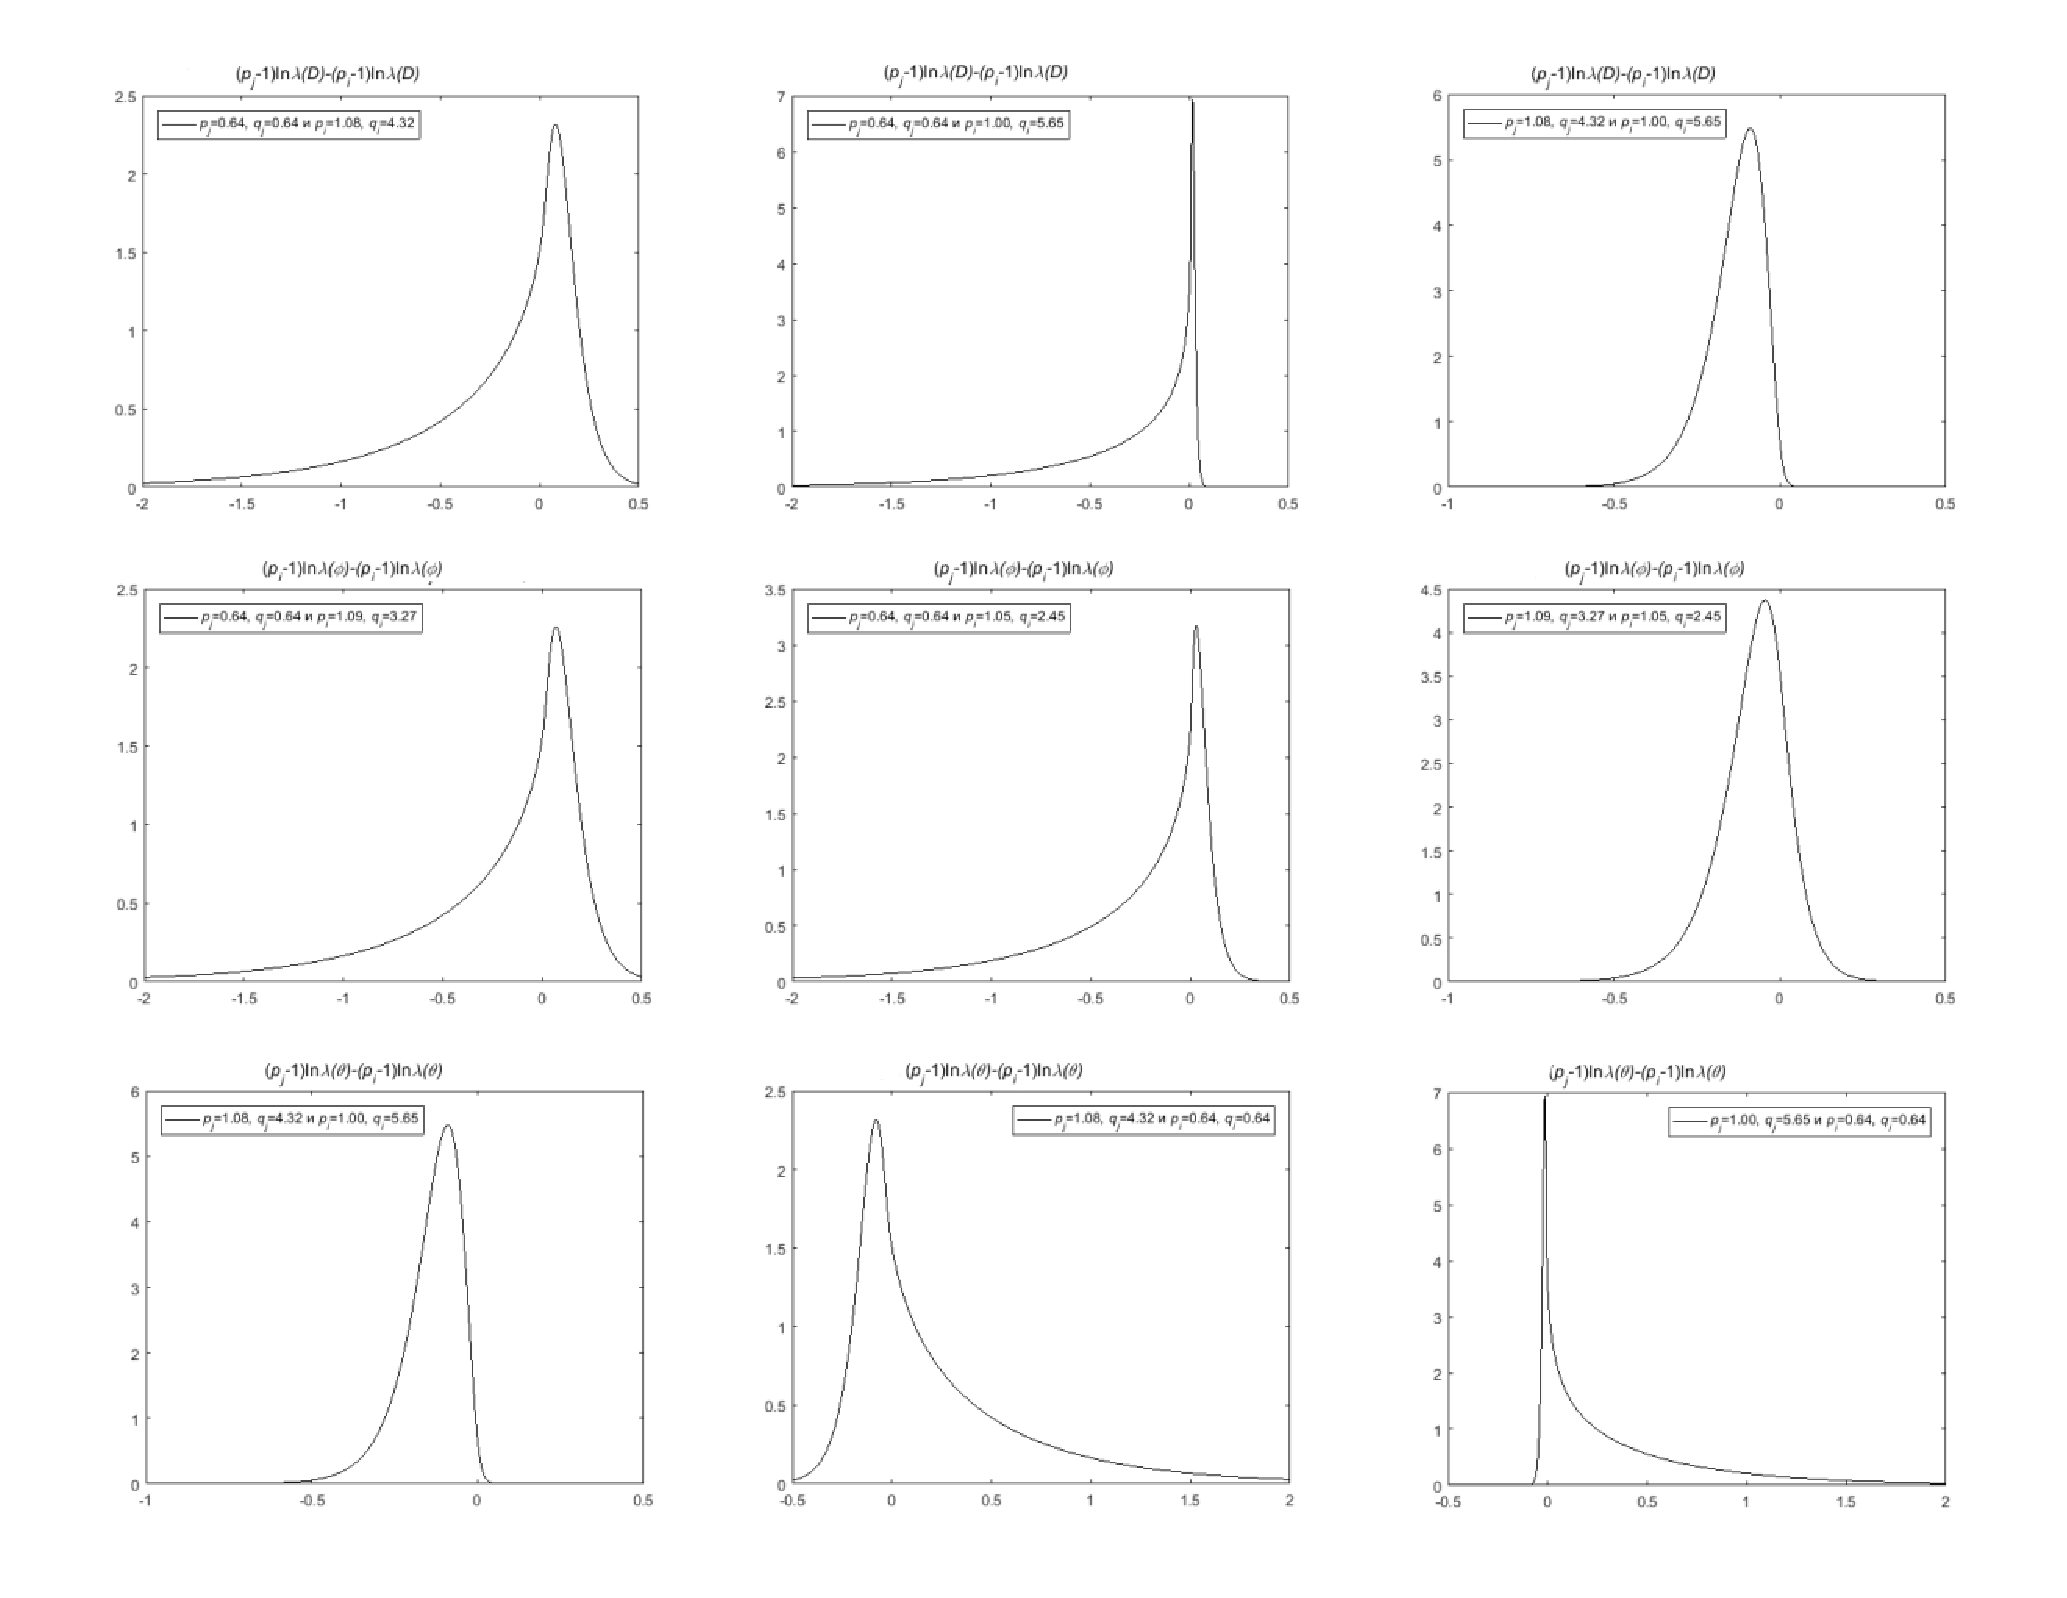
\includegraphics[width=1.0\textwidth]{pics/fig_3.pdf}
\captionstyle{normal}\caption{The laws of the distribution of statistics functions of maximum eigenvalue.}\label{fig:fig_3}
\end{figure}

\begin{figure}[h]
\setcaptionmargin{5mm}
\onelinecaptionstrue
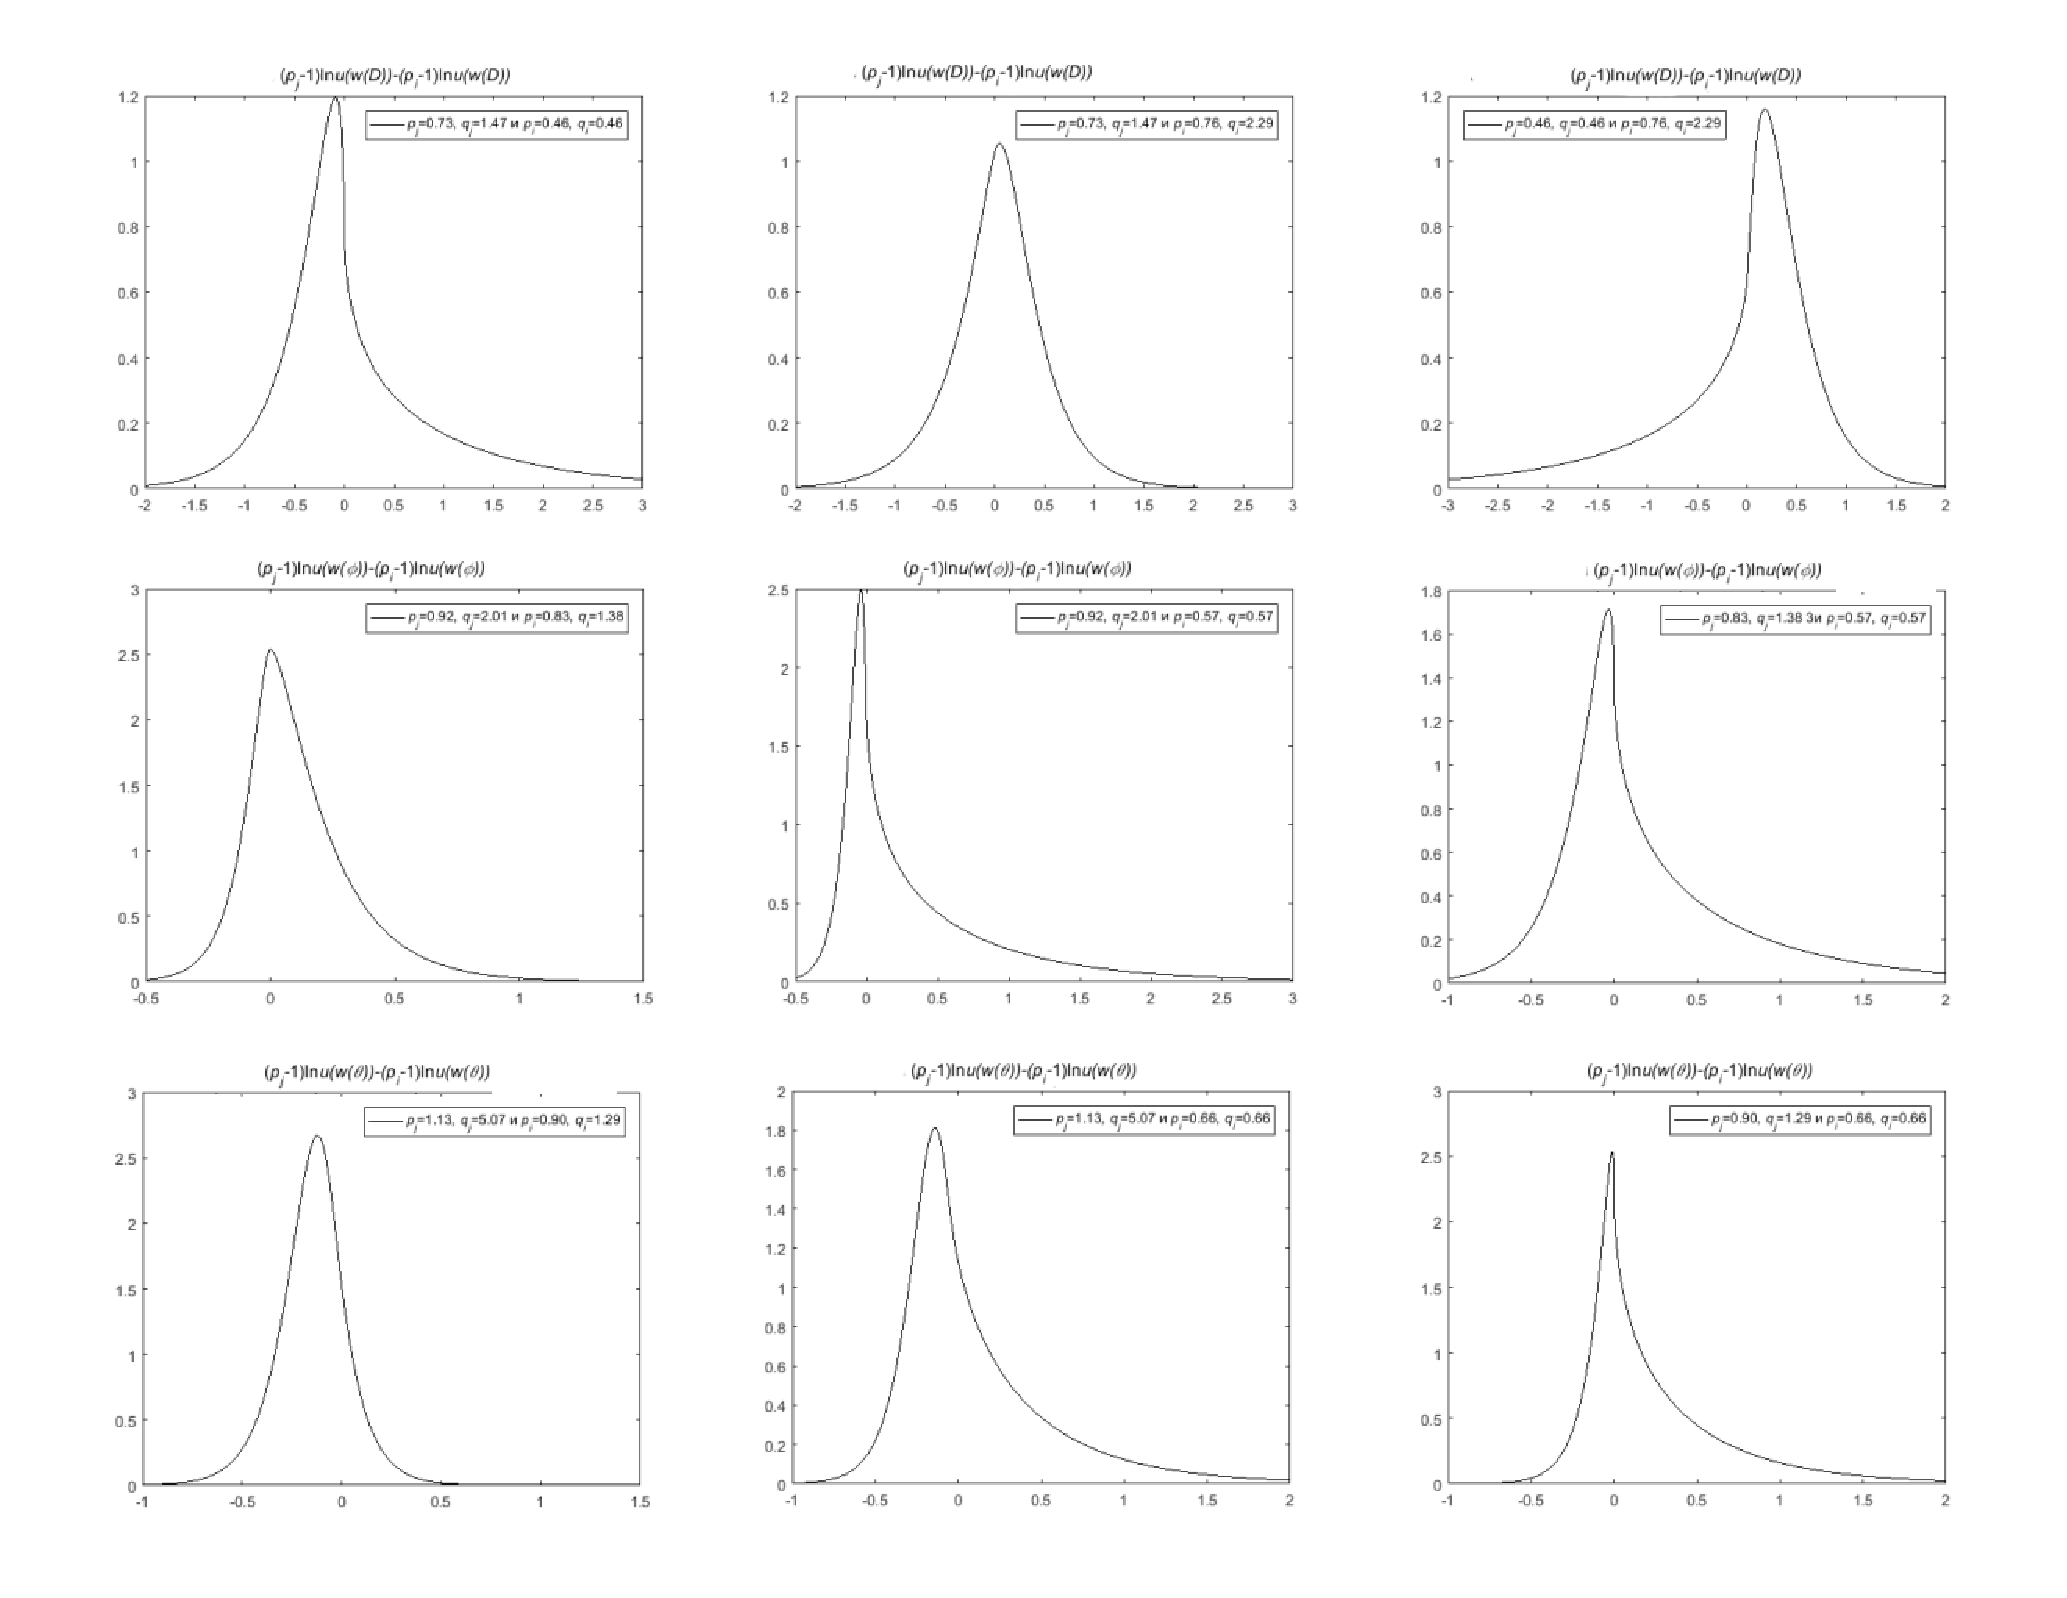
\includegraphics[width=1.0\textwidth]{pics/fig_4.pdf}
\captionstyle{normal}\caption{The laws of the distribution of the statistics functions of the energy of the wavelet spectrum.}\label{fig:fig_4}
\end{figure}
